\section{Parse Tree dan Abstract Syntax Tree (AST)}

\subsection{Parse Tree (Concrete Syntax Tree)}
Representasi visual lengkap dari derivasi string, termasuk semua terminal dan non-terminal pendukung.

\subsection{Abstract Syntax Tree (AST)}
Versi ringkas dari parse tree yang hanya menyimpan informasi esensial untuk tahap kompilasi berikutnya (semantik dan \textit{code generation}).

\begin{figure}[!htbp]
    \centering
    \adjustbox{max width=0.8\textwidth,center}{%
    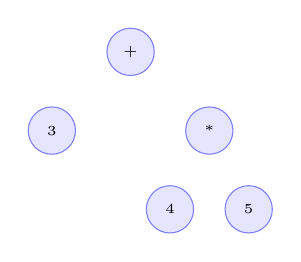
\begin{tikzpicture}[
        node/.style={circle, draw=blue!50, fill=blue!10, minimum size=0.6cm, font=\tiny}
    ]
    \node[node] at (0,0) {+};
    \node[node] at (-1,-1) {3};
    \node[node] at (1,-1) {*};
    \node[node] at (0.5,-2) {4};
    \node[node] at (1.5,-2) {5};
    \end{tikzpicture}%
    }
    \caption{Contoh struktur AST}
\end{figure}
